\documentclass[thesis=M,english,hidelinks]{FITthesis}[2012/10/20]



\usepackage[utf8]{inputenc}
\usepackage[T1]{fontenc}

% TYPOGRAPHY
\usepackage{inconsolata}
\usepackage{tgpagella}
\usepackage{PTSans}

% \DisemulatePackage{setspace}
% \usepackage{setspace}
% \onehalfspacing

\OnehalfSpacing

\setsecheadstyle{\bfseries\LARGE\sffamily}
\setsubsecheadstyle{\bfseries\large\sffamily}
\setsubsubsecheadstyle{\bfseries\normalsize\sffamily}

\newcommand{\code}{\texttt}

\definecolor{red}{HTML}{a31422}
\definecolor{green}{HTML}{00894e}
\definecolor{darkgray}{HTML}{3e3e3e}
\definecolor{gray}{rgb}{.4,.4,.4}
\definecolor{purple}{rgb}{0.65, 0.12, 0.82}

\usepackage{listings}
\lstset{
  basicstyle=\footnotesize\ttfamily\color{gray},
  breaklines=true,
  frame=lines,
  framexleftmargin=\parindent,
  framexrightmargin=\parindent,
  framextopmargin=\baselineskip,
  framexbottommargin=\baselineskip,
  aboveskip=\baselineskip,
  showspaces=false,
  showstringspaces=false,
  framerule=0.2pt
}

\lstdefinelanguage{JavaScript} {
  keywords={break, case, catch, continue, debugger, default, delete, do, else, false, finally, for, function, if, in, instanceof, new, null, return, switch, this, throw, true, try, typeof, var, void, while, with},
  morecomment=[l]{//},
  morecomment=[s]{/*}{*/},
  morestring=[b]',
  morestring=[b]",
  ndkeywords={class, export, boolean, throw, implements, import, this},
  keywordstyle=\color{red},
  ndkeywordstyle=\color{darkgray},
  identifierstyle=\color{darkgray},
  commentstyle=\color{purple},
  stringstyle=\color{green},
  sensitive=true
}

\usepackage{float}

\usepackage{graphicx}
\graphicspath{{img/}}
% \usepackage{subfig} %subfigures

\usepackage{dirtree}

% % list of acronyms
% %\usepackage[acronym,nonumberlist,toc,numberedsection=autolabel]{glossaries}

\department{Department of Software Engineering}
\title{Application for Entering and Evaluation of Written Exams}
\authorGN{Adam}
\authorFN{Havel}
\author{Adam Havel}
\authorWithDegrees{Bc. Adam Havel}
\supervisor{doc. Ing. Tomáš Vitvar, Ph.D.}
\acknowledgements{THANKS}
\abstractEN{}
\abstractCS{}
\placeForDeclarationOfAuthenticity{Prague}
\keywordsCS{Replace with comma-separated list of keywords in Czech.}
\keywordsEN{Replace with comma-separated list of keywords in English.}
\declarationOfAuthenticityOption{1} %select as appropriate, according to the desired license (integer 1-6)


\begin{document}

\setsecnumdepth{part}
\chapter{Introduction}

\setsecnumdepth{all}

\chapter{Analysis}

\chapter{Realization}

  \section{Server}

    \subsection{Architecture}

      \subsubsection{Structure}

    \subsection{Database}

    \subsection{Internal communication}

      \subsubsection{API}

      \subsubsection{Websockets}

\section{Client}

  \subsection{Architecture}

    \subsubsection{Structure}

    \subsubsection{Routing}

    \subsubsection{Services}

The core of the application lies in the so called services which are objects that are used to organize code into logical units and wired together using dependency injections to create new functionality. They are built upon services already present in Angular like \code{\$http} or \code{\$resource}  and are instantiated only when another component depends on them. The so called service factory then generates a single instance and provides a reference. Any other component that might require the same service will receive a reference to the same instance. Using this feature, data can be easily shared between different parts of the application.

Much of the core functionality is handled by aptly named services such as \code{ExamTake} or \code{NewBlueprint}. The user interface controller actually depends on many of these, so that it can provide information about their state to users. That is the reason most of the services get instantiated right at the initial load. Nonetheless, some of them are used only by a subset of users, depending on a user's role. That is why we want to know the role before we start creating instances of services a user might not be able to use anyway. Since the majority of the services also create event listeners, they would only pose as a potential memory hog.

This is where the \code{User} service comes in play. It is able to tell if a user is logged in and what is eventually his role and then provide that information to other components. If a user successfully authenticates, it emits a \code{loggedIn} message to \code{\$rootScope}---kind of a common ground for all components that depend on it. Any service listening will receive the message and inspect the value of the role in return. Knowing that information, it can safely decide whether to self-initialize or not.

    \subsubsection{Directives}

  \subsection{Optimization}

    \subsubsection{Task automation}

\section{Interface}

  \subsection{Design}

Taking the proposed use of the application into account, it is crucial to embrace the idea that the design might be the most important aspect of the product and also the ultimate measure of its reach and usefulness. And when talking about design, we mean not just the aesthetics, of course, but also the whole field of user experience and usability. It is no secret that dealing with a poorly designed product can actually become a source of stress by itself, or just a very unpleasant experience at best. The situation one finds himself in while trying to use such application usually only helps to heighten this feeling---and taking an exam can be quite gruelling as it is, as anyone can attest. Forcing students to use an application that is hard or simply obnoxious to use would epitomize nothing more than a major tell-tale sign of bad decision-making at every level of the design process.

    \subsubsection{Flat or skeuomorphic?}

As Dieter Rams once famously stated in his ten principles for good design (sometimes understandably referred to as the ``Ten commandments''), ``good design is as little design possible.'' And even though Rams dealt mostly with product design, the statement is applicable everywhere. Less, but better---such design can concentrate on the essential aspects instead of burdening the product with non-essentials. In recent years, this minimalist approach has once again proved to be in good health when the so called ``flat'' design seized the reins of user interface design everywhere. The reason it is referred to as flat is because it removes any stylistic choices that give the illusion of three-dimensionality (such as drop shadows, gradients, or textures) and focuses on simple elements, typography and primary colors.

In opposition to flat design lies what is called skeuomorphism. Essentially any interface using ornamental cues referring to an object in the physical world is said to be skeuomorphic. These cues are intended to help the user navigate the interface by creating a sense of familiarity. Among the many arguments against skeuomorphic design are those which state that skeuomorphic interface elements use metaphors that are more difficult to operate and take up more screen space than standard interface elements or that many users may have no experience with the original device they emulate. Also prevalent is the opinion that such design limits creativity by grounding the experience to physical counterparts.

Valid or not, these arguments helped pave the way for the domination of flat design. One does not have to look far for evidence---take for example the design of \textit{Windows 8} and compare it to previous versions. Then do the same with \textit{iOS 7}. The trend's existence is indisputable---but it is the author's belief that as with any trend, it is best not to get carried away and trust one's judgement first. It is undeniable that flat design allowed interface designs to be more streamlined and efficient, and to quickly convey information while still looking visually appealing and approachable. However, when used without questions and reservation, it can actually obfuscate the meaning behind an interface.

\begin{figure}
  \setlength\fboxsep{0pt}
  \setlength\fboxrule{0.2pt}
  \fbox{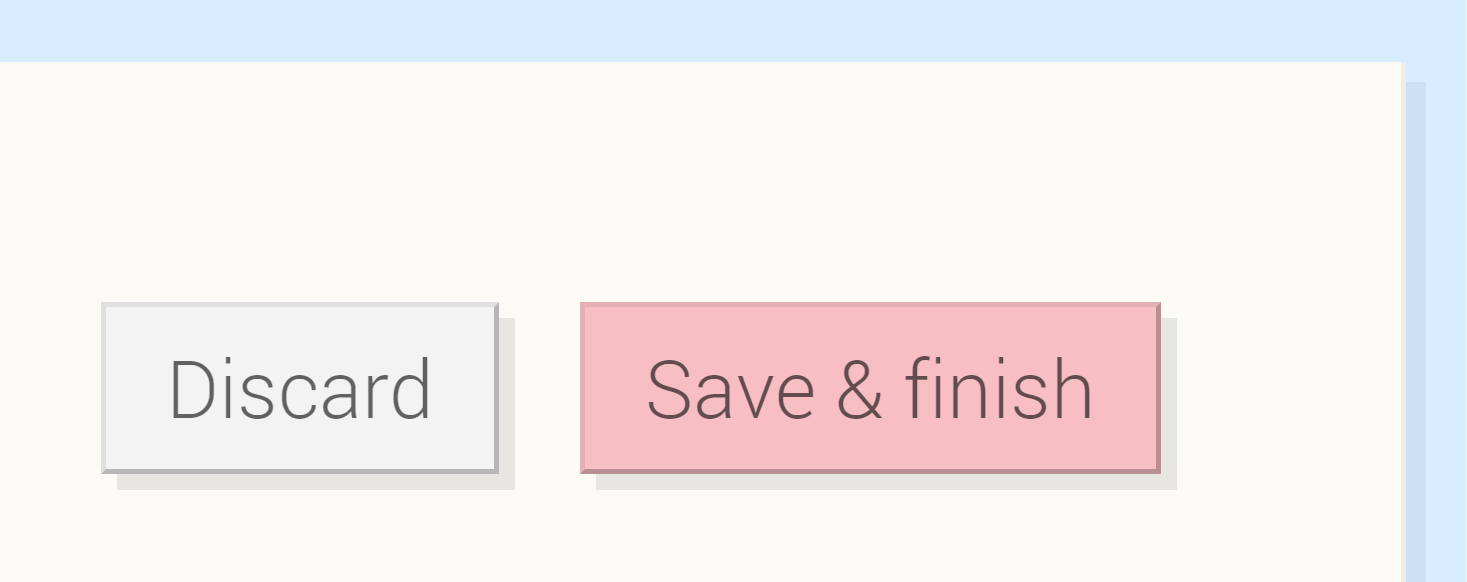
\includegraphics[width=\textwidth]{buttons.png}}
  \caption{Example of buttons}
  \label{fig:buttons_example}
\end{figure}

This is what Dieter Rams meant when he said that good design makes a product understandable. We can take the cornerstone element of every interface---a button---and use it as a kind of guinea pig. If we blindly followed the principles of flat design (which many do), the element's visual identity would quickly fall apart. But say we add a simple drop shadow---the metaphor then holds and so do the streamlined aesthetics. The point is that the button does not have to look exactly like a button to be recognized as one. Giving the user a cue is usually enough, his mind will do the rest and fill the gaps. The same applies for an input element---the user expects it to have at least a slight inset drop shadow and is confused when the element is not given one. This has been proven time and again by many usability studies.

\begin{figure}
  \setlength\fboxsep{0pt}
  \setlength\fboxrule{0.2pt}
  \fbox{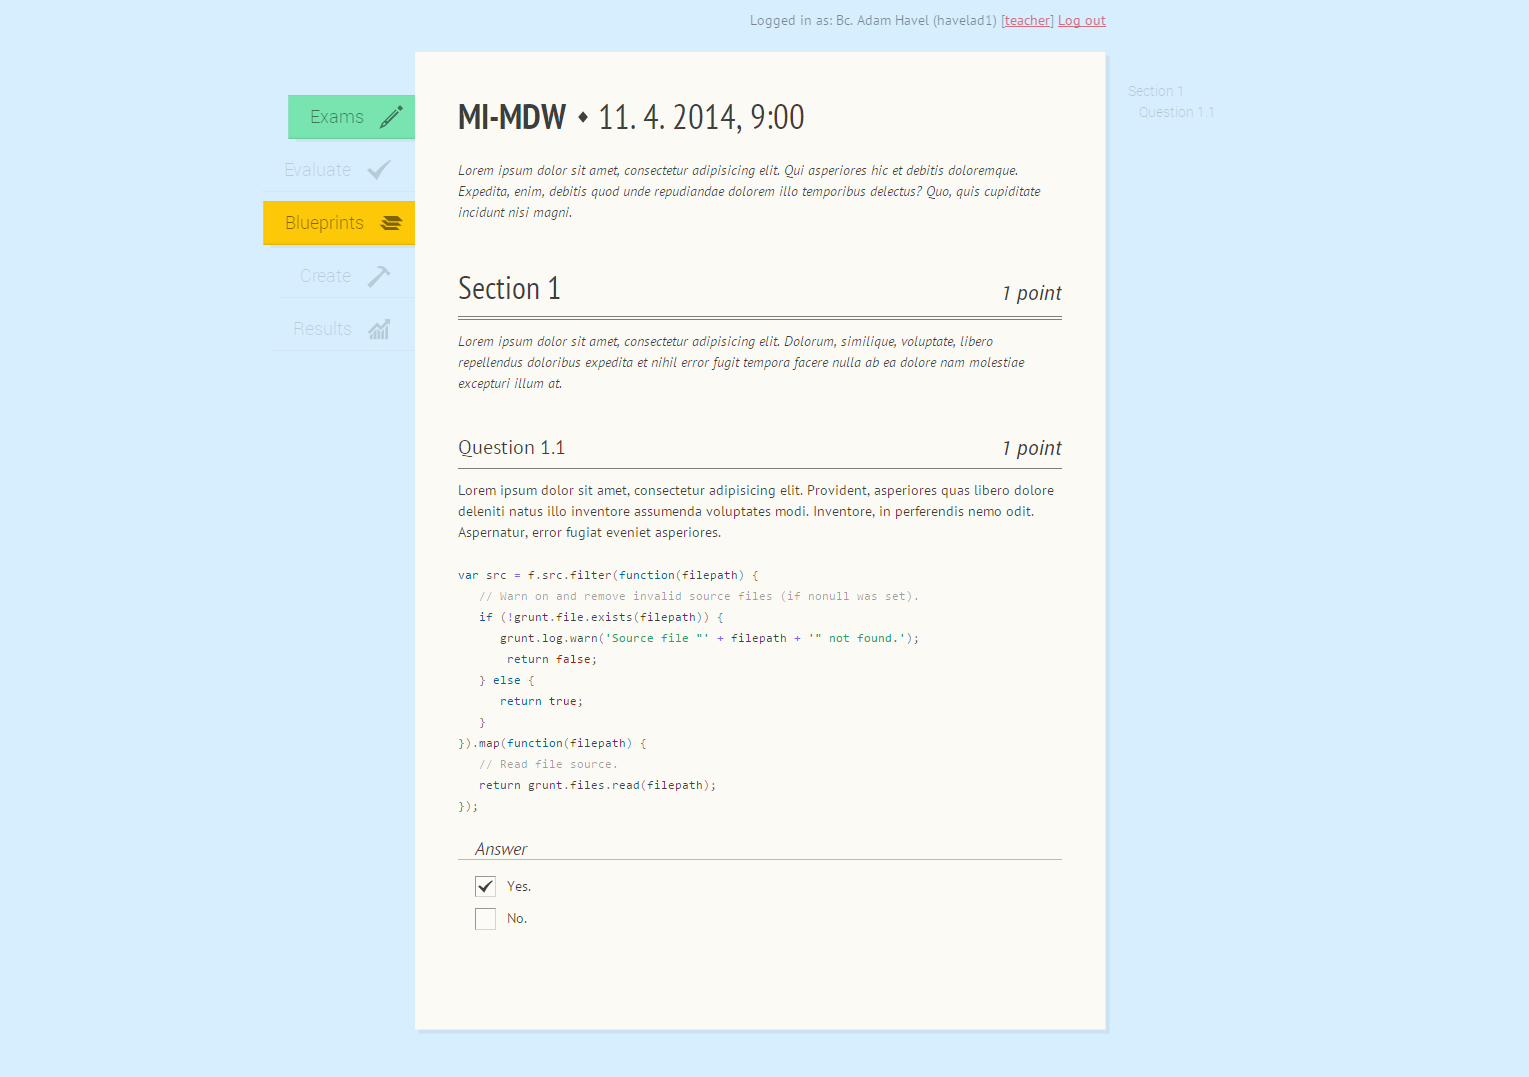
\includegraphics[width=\textwidth]{page.png}}
  \caption{Page layout}
  \label{fig:page_layout}
\end{figure}

It is because of these and many other reasons that the approach taken in designing the application user interface, while based on the principles of flat design in its focus on typography and color, is not shying away from some of the more reasonable aspects of skeuomorphism. Even though the design does rely heavily upon simple shapes and deliberate use of color, the most ostentatious attempt at emulating reality is immediately apparent when one takes a look at the page layout, as seen in the figure \ref{fig:page_layout}. The main content is presented in a form reminiscent of a sheet of paper. This is heightened by the use of color, a subtle drop shadow and the fact that when there is not enough content to stretch it further, the ``sheet'' holds a ratio of 1:1.414, the same as a real piece of paper. The reasoning behind this idea is to provide the users---especially the students---with something familiar. Novelties and surprises have their place in design, but one must choose wisely how and when to introduce them---confounding a student who is probably already struggling with his exam is hardly a good idea.

The side effect of this decision takes shape in the relatively small portion of the available viewport width being occupied by the main content, at least on displays designated for desktop use. This further strengthens the idea that the main content should always be in the spotlight. Any additional information that might not be essential but proves helpful is placed outside of this area---its opacity reduced unless in focus, in order not to distract the user. An example of such component is a table of contents which, apart from providing the document structure at a quick glance, allows an user to tell his current position and to swiftly jump to a different part by way of anchor links.

Menu

    \subsubsection{Typography}

    \subsubsection{Colors}

The backdrop color has been chosen deliberately for its properties and effects on human mind. A light that is composed predominantly of the color blue has a direct and powerful influence on the secretion of melatonin, a hormone that regulates sleep patterns in mammals. So while it is generally a good idea to avoid blue light at night in order not to disturb one's sleep, the very same quality can be used during the day to effectively raise a person's alertness.

While other colors might not have the same powerful properties, each of them holds some kind of meaning, which is more often than not defined by culture. It would therefore be unwise not to follow these leads and use the colors haphazardly. One simply has to know its product's target market and adjust accordingly to local traditions. Little details such as the fact that in the Japanese culture, the color white represents death may seem peculiar for us Westerners, but in the end do matter.

As already mentioned, the main content is filled with an off-white color expressed as a RGB hex triplet with a value of \code{\#fbfaf5}. Apart from trying to mimick the properties of a real paper, such color tends to be easier on eyes than pure white. The other colors in use are employed mainly as a visual cue so that a user can quickly grasp the meaning behind a message or a prompt. This is especially true for the so called modal windows, which are leaned upon heavily in the application. A modal window is a kind of a child window that requires a user interaction in order to allow the user to return to the main window. They are used to draw attention to vital pieces of information or to display emergency states. And even though they are often criticized for breaking a user's workflow, more often than not, they

    \subsubsection{Icons}

    \subsubsection{Performance}

\chapter{Processes}

  \section{Authentication}

No part of the system is accessible without authentication. Upon loading, the client makes a \code{GET} request to a resource defined at \code{/api/user} and appends a session identifier if a cookie is found. The server then tries to look up the identifier in MongoDB-backed session store. If successful, it checks whether the session has not expired---if that is not the case, it sends the client a JSON object containing information about the particular user. The information is obtained by deserializing the user identifier from the session and using it to fetch relevant data from the database. The client application then fills its \code{User} service with the received object and the user is onward recognized as authenticated.

    \subsection{Logging in}

In the opposite case---either no session was found or it has already expired---the server responds with a 401 status code which forces the client to show the user to a login form. After filling in the form, the client makes a new request to the \code{api/user} resource, this time using the \code{POST} method, sending along user credentials. These credentials are then checked against a faculty LDAP server running at \code{ldap.fit.cvut.cz} using a secure connection. If user's identity is verified, the LDAP server responds with basic information about the user. Back at the application server, the database is queried for additional data using the user identifier. It either finds a relevant entry or not. In the former case, the entry is updated with a new timestamp, representing the last login time, and the server sends it to the client as a JSON object, the same as before. If the latter is the case, it means that the user is logging in for the first time.

\begin{figure}
  \setlength\fboxsep{0pt}
  \setlength\fboxrule{0.2pt}
  \fbox{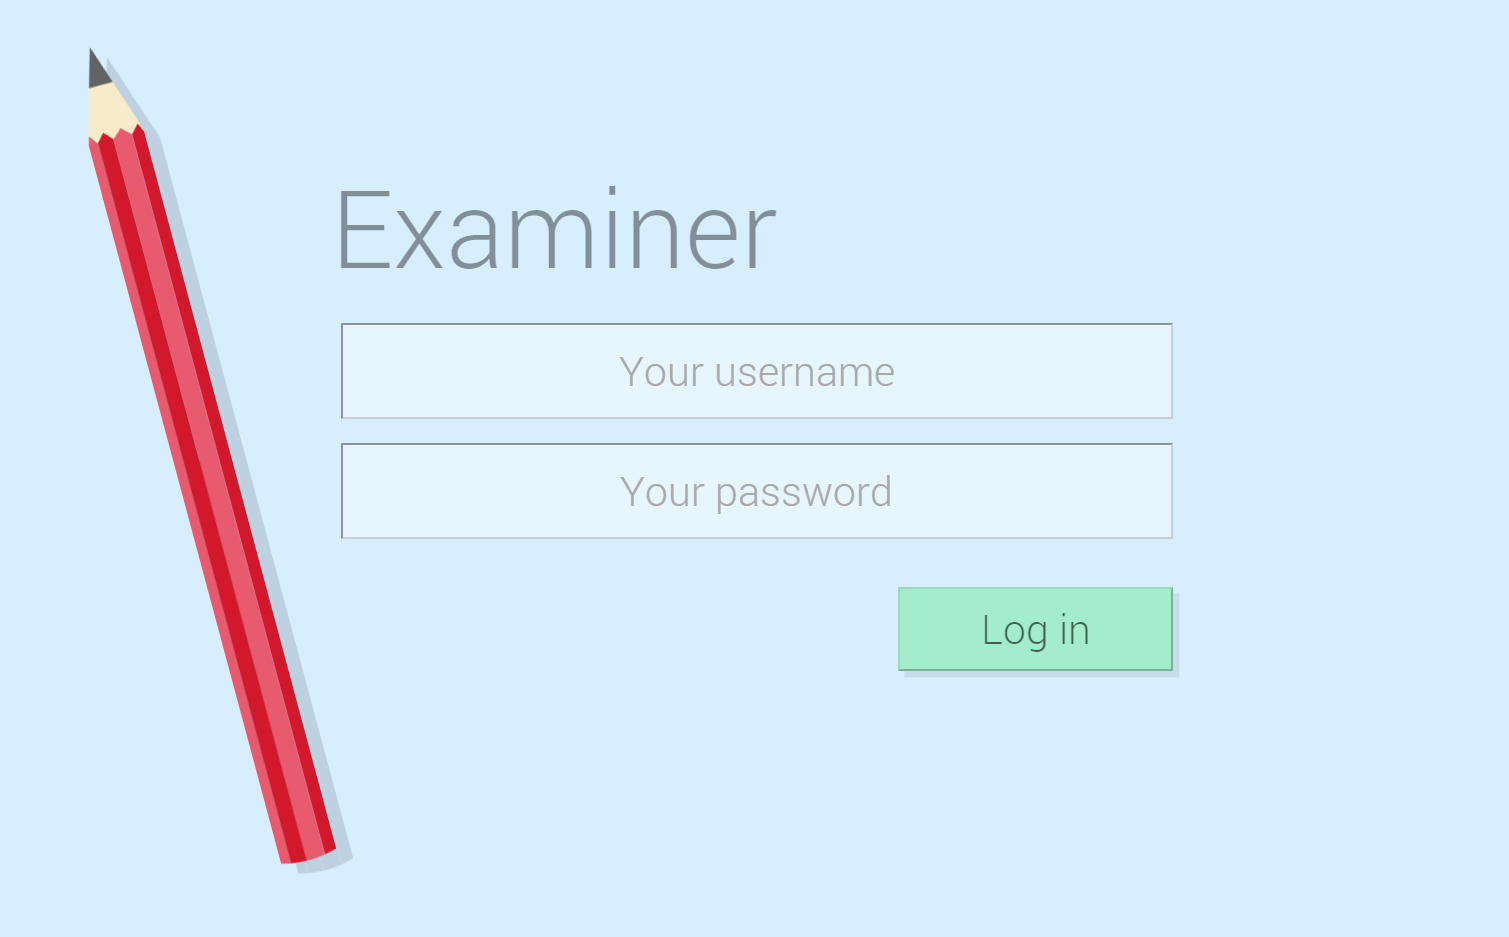
\includegraphics[width=\textwidth]{test.png}}
  \caption{Login form}
  \label{fig:login_form}
\end{figure}

A new instance of \code{User} model is then created and filled with the available data. What remains unknown is the user's role---that is, if he or she is a student or a teacher. That information can be obtained by making a request to \textit{KOSapi}, a faculty service that provides a REST API over the university information system \textit{KOS}. To find out the role of a person with a given user identifier we can utilize the resource \code{/people/\{uid\}}. With that issue resolved, we can continue by looking up all courses the user either studies or teaches by using the resources \code{/students/\{uid\}/enrolledCourses} and \code{/teachers/\{uid\}/courses}, respectively. It is worth noting that \textit{KOSapi} returns the data formatted as XML, which means the server has to transform it into a JSON object, for which it uses an external library called \textit{x2js}. After obtaining all the necessary data, the new user can finally be saved in the database and sent to the client.

But since both the role and the subjects of a user can change, the server has to periodically request the current states of the aforementioned resources and make necessary changes in the application database. This is one of the reasons the last login time is saved in the \code{User} model---using this information, the server makes sure not to ask for new data more than once a day. And since the majority of these changes occur at the start of a semester, long before any exam takes place, it should be frequent enough for most cases.

    \subsection{Client-side verification}

When the client receives the authentication data and stores it in the appropriate service, the user can start to use the application with the scope assigned to his role. If for some reason the \code{User} service gets unset again, the user is shown a login form and any navigation elsewhere is disabled until he successfully logs in. In this manner, the authentication is verified only via the client-side service which might not be up to date with the server. This is sufficient for some operations and serves to mitigate any latency that would arise from communication between the client and the server.

If the user logs out, the \code{User} service is emptied and the client sends a \code{DELETE} request to the \code{/api/user} resource which prompts the server to discard the session. Nonetheless, the client session might also be terminated at the server end, either by force or because it has expired. It is therefore necessary that the client recognizes this situation and acts accordingly. This is ensured by using a HTTP interception service that monitors every response the client receives from the server when it tries to reach a resource. Whenever a 401 status code shows up, it means the session has been ended and the user has to authenticate again if he wishes to continue.

\begin{figure}[h]
  \begin{lstlisting}[language=JavaScript]
app.factory('AuthInterceptor', function($q, $injector, Modal) {

  return {
    'response': function(response) {
      if (response.status === 401 && $injector.get('User').data) {
        Modal.open('alert', 'Your session has been ended. You will have to authenticate.', null, 'Log in');
        $injector.get('User').logout();
        return $q.reject(response);
      } else {
        return response || $q.when(response);
      }
    }
  };

}).config(function($httpProvider) {
  $httpProvider.interceptors.push('AuthInterceptor');
});
  \end{lstlisting}
  \caption{HTTP Interceptor}
  \label{fig:http_interceptor}
\end{figure}

The HTTP interceptor can be seen in the figure \ref{fig:http_interceptor}. It requires the \code{User} service so that it can tell whether a user is present and to log him out if necessary. In any other type of component, the \code{User} service would be injected normally, but that is unfortunately not possible in this scenario. The problem arises from the fact that injecting a service into another component makes it dependent on that service. And since the \code{User} service is already dependent on \code{\$http} and applying the interceptor essentially modifies the instance of the very same \code{\$http}, making \code{\$http} dependent on the \code{User} service through the interceptor would create what is called a circular dependence. That can be remedied by using the built-in \code{\$injector} service which is able to get hold of another service reference without creating a dependence.

Something similar to the 401-filled responses also occurs when a user is not authorized to view a selected resource. This applies for example in the case when a user with the role of a student requests a different student's results. When such a thing happens, the server responds with a status code 403. Nevertheless, such request is never made on behalf of the client application and can only occur when the user tries to reach the server resource directly, via the provided API. That is why we do not have to handle this problem on the client side.

  \section{Blueprints}

A blueprint represent what in real life would be the original copy of a written test. In the application, blueprints can be created, viewed and modified until the day of the exam. Quite obviously, all of these operations are allowed only for users that hold the role of a teacher. And even those can manage only the blueprints that belong to the courses they teach.

    \subsection{Resources}

The blueprints are exposed as two resources, each of them designed for different use. The first one represents a collection of blueprints and is accessible via \code{/api/blueprints}. It supports optional query parameters for filtering by subject, date and language. When no subject is specified, the result is automatically filtered using the list of subjects contained in the \code{User} service. If, on the other hand, a subject is given, it is tested against the same list and if no match is found, the server responds with a 403 code. Otherwise, the query is passed along.

In the end, the resource returns a collection of all the blueprints in the database that satisfy the inherent or supplied conditions. Anyhow, since the resource is used only for listings on the client side, it is unreasonable to request the actual content of the blueprints. Sending just the basic information will suffice and anything more than that would be a waste of bandwidth. To trim the response, the client can use the optional parameter \code{fields}. It is available to all the resources the API provides and when given, it prompts the server to return only the specified fields.

The other resource is used for operations dealing with a particular blueprint and can be found at URI \code{api/blueprint/\{subject\}/\{date\}/\{language\}}. Note that the variables are not optional and must be validated before any further processing, otherwise the server returns an error. The subject must be a valid subject code---starting with either \code{MI} or \code{BI} depending on the level of the subject, followed by a hyphen and ending with three word characters. The date must represent a string formatted as \code{YYYY-MM-DDThh:mm}, for example \code{2014-04-25T07:51}, and the language is validated against the standard \textit{ISO 639-1} which allows only codes like \code{en} or \code{cs}.

The combination of these three variables is the only unique identifier of a blueprint in the application. There is a different type of key we might have used, which is the entry identifier assigned to every exam term in \textit{KOS}, but because of the fact that an exam can be taken in different languages at once, it would not suffice. Even though such case is not very probable, it could still happen, and there is no reason for the application not to be as flexible as possible. It also helps retain a certain human-friendliness, as opposed to having to query the server API using generated identifiers.

    \subsection{Viewing blueprints}

To view the blueprints, which only teachers are allowed to, the user must navigate to the state \code{Blueprints} which results in URL \code{/blueprints}. The items depicted are organized in stacks which reflect the logical distribution of blueprints among subjects. If only one subject is available, the user is presented directly with individual blueprints. Clear graphical distinction is made between what is considered stack and what is an individual ``sheet'' so that the user quickly recognizes which is which. Apart from using the browser history, the user can navigate the blueprints using a breadcrumbs navigation. This is possibly excessive in this case but makes more sense in different listings, for example when viewing exams where the structure depth can reach four levels. Also important is the fact that the current level is shared among all listings, which should help with the workflow. Anyhow, the listing is empty so far because we have yet to create our first blueprint.

    \subsection{New blueprint}

To create a new blueprint, the user must enter the state \code{NewBlueprint} which is reflected in the URL as \code{/new}. She is then presented with a listing similar to the one before, only this time with exam terms instead of blueprints. Terms are the particular dates on which an exam takes place---we can get those by reaching the \textit{KOSapi} resource \code{/courses/\{subject\}/exams}, using each of the user's subjects as the variable. The client actually asks the application server resource \code{api/examterms/\{subject\}} whose only job is to delegate the request to the aforementioned endpoint and return the transformed result. But before sending the request

    \subsection{Modifying blueprint}

  \section{Exams}

    \subsection{Viewing exams}

    \subsection{Ongoing exams}

      \subsubsection{Watching over exams}

      \subsubsection{Taking exams}

    \subsection{Exam evaluation}

\setsecnumdepth{part}
\chapter{Conclusion}


\bibliographystyle{iso690}
\bibliography{mybibliographyfile}

\setsecnumdepth{all}
\appendix

\chapter{Acronyms}

\begin{description}
   \item[API] Application Programming Interface
   \item[HTTP] Hypertext Transfer Protocol
   \item[JSON] JavaScript Object notation
   \item[LDAP] Lightweight Directory Access Protocol
   \item[REST] Representational State Transfer
   \item[XML] Extensible Markup Language
\end{description}


\chapter{Contents of enclosed CD}

\begin{figure}
   \dirtree{%
      .1 readme.txt\DTcomment{the file with CD contents description}.
      .1 exe\DTcomment{the directory with executables}.
      .1 src\DTcomment{the directory of source codes}.
      .2 wbdcm\DTcomment{implementation sources}.
      .2 thesis\DTcomment{the directory of \LaTeX{} source codes of the thesis}.
      .1 text\DTcomment{the thesis text directory}.
      .2 thesis.pdf\DTcomment{the thesis text in PDF format}.
      .2 thesis.ps\DTcomment{the thesis text in PS format}.
   }
\end{figure}

\end{document}
